\documentclass{beamer}
\mode<presentation>{
  \usetheme{boxes}
}


\usepackage[T1]{fontenc}
\usepackage[utf8]{inputenc}
\usepackage[swedish]{babel}
\usepackage{epstopdf}
\usepackage{array}

\usepackage{listings}
\usepackage{graphics}
\usepackage{tikz}
\usepackage{comment}
\usetikzlibrary{trees,arrows,automata}

\usepackage{wasysym}
\usepackage{fancyvrb}
\DefineVerbatimEnvironment{code}{Verbatim}{fontsize=\small}
\DefineVerbatimEnvironment{example}{Verbatim}{fontsize=\small}
\newcommand{\ignore}[1]{
}

\lstnewenvironment{codeEx}
{\lstset{ basicstyle= \ttfamily }}
{}

\lstnewenvironment{codeExDiff}
{\lstset{ basicstyle=\color{black} \ttfamily
        , moredelim=[is][\color{red}]{\#}{\#}
        } }
{}

\newcommand{\sepFrame}[1] {
\begin{frame}
\begin{center}
	\Huge{#1}
\end{center}
\end{frame}
}

\newcommand{\ndist}{1.7cm}
\newcommand{\nshift}{0.8cm}
\newcommand{\nshiftw}{1.2cm}
\newcommand{\ncol}{blue!20!white}
\newcommand{\lcol}{red!20!white}

\newcommand{\tree}[5] {
\begin{figure}[H]
    \centering
        \begin{tikzpicture}[->,node distance=\ndist, semithick]
        	\tikzstyle{every node}=[
                                minimum width=1.4cm
                                ,minimum height=0.7cm]
            \node[draw,fill=\ncol](add) {#2};
            \node[draw,fill=\ncol](mul)[below of=add, xshift=\nshiftw] {#3};
            \node[draw,fill=\ncol](sin)[below of=add, xshift=-\nshiftw] {#1};
            \node[draw,fill=\lcol](x1)  [below of=sin, xshift=0cm] {#4};
            \node[draw,fill=\lcol](x2)  [below of=mul, xshift=-\nshift]  {#4};
            \node[draw,fill=\lcol](five)[below of=mul, xshift=\nshift]  {#5};
            \path (add) edge node {} (mul)
                        edge node {} (sin)
                  (mul) edge node {} (x2)
                        edge node {} (five)
                  (sin) edge node {} (x1);
        \end{tikzpicture}
\end{figure}

}

\newcommand{\haskellcol}{red!20!white}
\newcommand{\ourcol}    {blue!20!white}
\newcommand{\stgcol}    {purple!20!white}
\newcommand{\runcol}    {green!20!white}


\usepackage{listings}
\usepackage{tikz}

\lstset{escapechar=\%}

\tikzstyle{every picture}+=[remember picture]
\tikzstyle{na} = [baseline=-.5ex]



\begin{document}

\title{Optimering under körningstid}

\author{Simon Edwardsson \and Olle Fredriksson
\and \linebreak{}
Daniel Gustafsson \and Dan Rosén}


\institute{Chalmers Tekniska Högskola\and Göteborgs Universitet}

\everymath{\displaystyle}

\begin{frame}
    \titlepage
\end{frame}
\begin{frame}

	%Vad sysslar vi egentligen med (vart befinner vi oss) (graf fran olle) 
	\begin{figure}[H]
        \begin{tikzpicture}[scale=0.7,transform shape,->,rounded corners
                           ,auto,node distance=3.2cm, semithick]
        \tikzstyle{every state}=[fill=\haskellcol
                                ,rectangle
                                ,minimum size=2.0cm]
		\path[use as bounding box] (-4,-2) rectangle (10,-2);
        \node<1->[state](haskell)[]                   {Haskell};
        \node<2->[state,fill=\stgcol](stg)    [below of=haskell]                   {STG-kod};
        \node<3->[state,fill=\ourcol](socker) [left of=stg]        {Sockerkod};
        \node<4->[state,fill=\runcol](int) [right of=stg,xshift=3.0cm] {
          \begin{tikzpicture}[semithick]
            \node<4->[state,fill=\ourcol](stgint) [right of=stg]       {STG-tolk};
            \node<5->[state,fill=\ourcol](opt)    [right of=stgint]    {Optimering};
            \path<5->
              (stgint) edge[bend left] node {} (opt)
              (opt)    edge[bend left] node {} (stgint);
          \end{tikzpicture}
          Körning
        };
        \path<3-> (socker) edge            node {} (stg);
        \path<4-> (stg)    edge            node {} (int);
        \path<2-> (haskell) edge           node {} (stg);
    \end{tikzpicture}
\end{figure}

\end{frame}



\begin{frame}
\begin{figure}[H]
\centering
    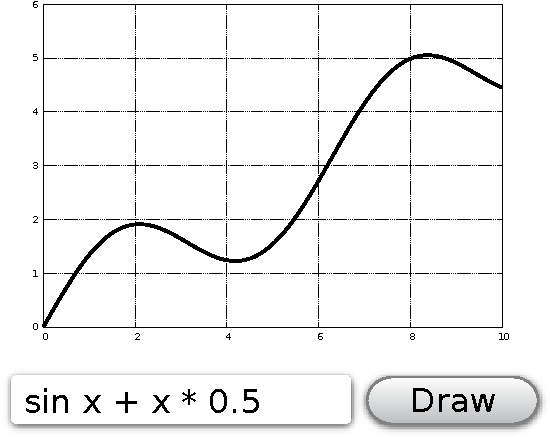
\includegraphics{img/draw.pdf}
\end{figure}

\end{frame}

\begin{frame}[fragile]
\centering
\begin{tabular}{ m{3.5cm} m{0.5cm} m{5cm} }
    \verb|"sin(x) + x * 0.5"| &  $\Rightarrow$
    &
	\tree{sin}{+}{*}{x}{0.5}
\\
\end{tabular}
\end{frame}

\begin{frame}[fragile]
\centering
\begin{tabular}{ m{3.5cm} m{0.5cm} m{5cm} }
    \verb|"sin(x) + x * 0.5"| & $\Rightarrow$
    &
	\tree{Sin}{Add}{Mul}{Var}{Num 0.5}
\\
\end{tabular}
\end{frame}

\begin{frame}[fragile]
\centering
\begin{tabular}{ m{10cm} }
\tree{Sin}{Add}{Mul}{Var}{Num 0.5} \\
\begin{codeEx}
eval :: Expr -> Double -> Double
eval (Add l r) x = eval l x + eval r x 
eval (Sin e)   x = sin (eval e x)
eval Var       x = x
..
\end{codeEx}
% eval (Num n)   x = n
% eval (Mul l r) x = eval l x * eval r x
\\
\end{tabular}
\end{frame}

\begin{frame}[fragile]

%Bild på en graf, där vi visar att det finns många olika x värden. Här säger vi också att det finns ett problem.
\begin{codeEx}
map (eval expr) [-10..10]
\end{codeEx}

\end{frame}

\begin{frame}[fragile] 
\begin{codeExDiff}
map (#optimise# (eval expr)) [-10..10]
\end{codeExDiff}

\pause

\verb|eval' :: Double -> Double|
\pause
\verb|eval' x = eval (Add (Sin Var) (Mul Var (Num 0.5))) x|
\pause
\verb|eval' x = eval (Sin Var) x + eval (Mul Var (Num 0.5)) x|
\pause
\verb|eval' x = sin (eval Var x) + eval (Mul Var (Num 0.5)) x|
\pause
\verb|eval' x = sin x + eval (Mul Var (Num 0.5)) x |
\pause
\verb|...                          |

\verb|eval' x = sin x + x * 0.5|
%\end{verbatim}

\pause

\begin{codeExDiff}
map #eval'# [-10..10]
\end{codeExDiff}
\end{frame}



% knyta an till f;rra presentationen utan att utesluta de nya, kort namna att vi optimerar saker och forklarar ett vi nu ska ge ett exempel dar det ar anvandbart


\begin{frame}
	\begin{figure}[H]
        \begin{tikzpicture}[scale=0.7,transform shape,->,rounded corners
                           ,auto,node distance=3.2cm, semithick]
        \tikzstyle{every state}=[fill=\haskellcol
                                ,rectangle
                                ,minimum size=2.0cm]
		\path[use as bounding box] (-4,-2) rectangle (10,-2);
        \node[state](haskell)[]                   {Haskell};
        \node[state,fill=\stgcol](stg)    [below of=haskell]                   {STG-kod};
        \node[state,fill=\ourcol](socker) [left of=stg]        {Sockerkod};
        \node[state,fill=\runcol](int) [right of=stg,xshift=3.0cm] {
          \begin{tikzpicture}[semithick]
            \node[state,fill=\ourcol](stgint) [right of=stg]       {STG-tolk};
            \node[state,fill=\ourcol](opt)    [right of=stgint]    {Optimering};
            \path
              (stgint) edge[bend left] node {} (opt)
              (opt)    edge[bend left] node {} (stgint);
          \end{tikzpicture}
          Körning
        };
        \path (socker) edge            node {} (stg);
        \path (stg)    edge            node {} (int);
        \path (haskell) edge           node {} (stg);
    \end{tikzpicture}
\end{figure}

\end{frame}

\sepFrame{Demo}

\sepFrame{Användningsområden}

\begin{frame}
%\frametitle{Användningsområden}

\begin{tabular}{ m{5.5cm} m{4cm} }

\begin{itemize}
	\item Regular expressions
	\item Vetenskapliga beräkningar % dotproduct, power, newtonraphson, simuleringar
	\item Raytracer
\end{itemize}
&
\begin{figure}[H]
\centering
    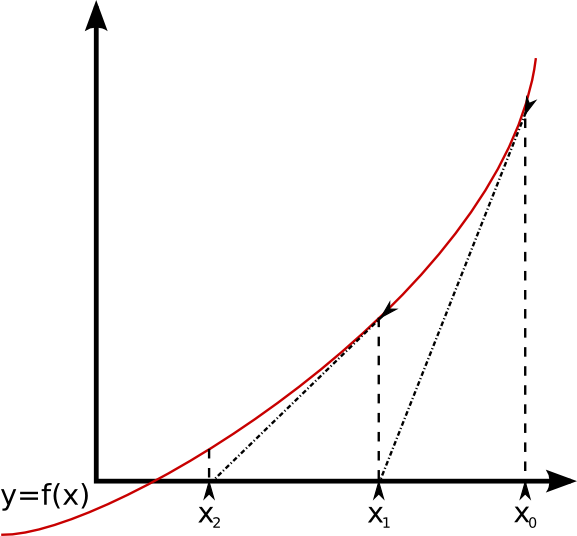
\includegraphics[width=0.5\textwidth]{img/metod.png} 

\end{figure}

\end{tabular}


\end{frame}
\begin{comment}
\begin{frame}
\begin{figure}[H]
\centering
    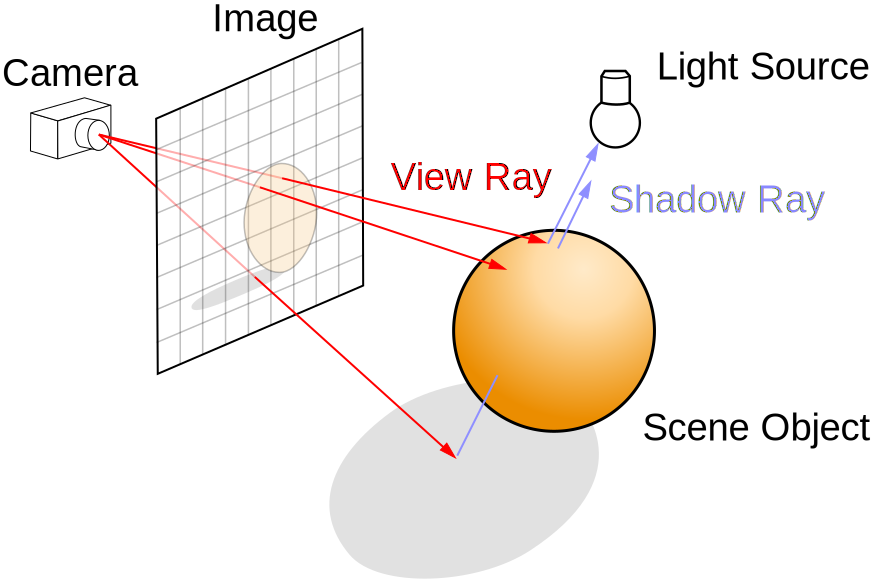
\includegraphics[width=1\textwidth]{img/Ray_trace_diagram.pdf} 
\end{figure}

\end{frame}
\end{comment}

\begin{frame}


\begin{figure}[H]
\centering
    
\includegraphics[width=0.6\textwidth]{img/shapes.png} 
\end{figure}


\end{frame}
\begin{frame}
\begin{figure}[H]
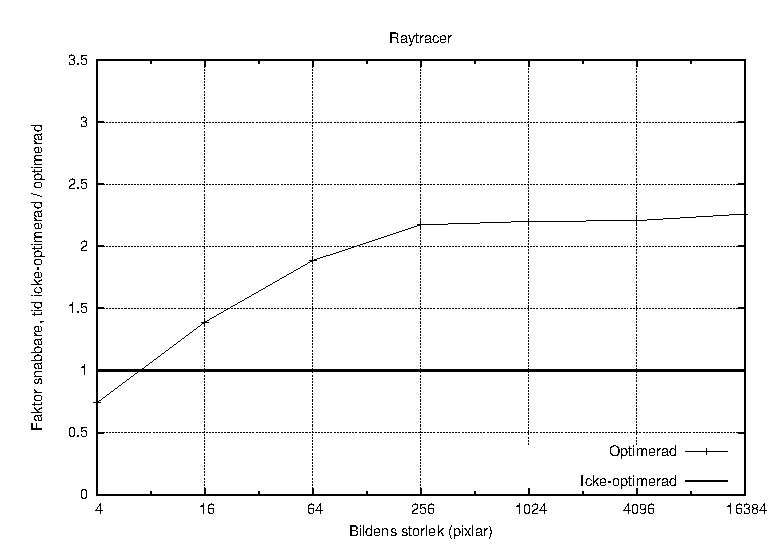
\includegraphics[width=1\textwidth]{shapesnormnocb.eps}
\end{figure}


\end{frame}

\begin{comment}
\begin{frame}

	Gobby 

\end{frame}
\end{comment}

\sepFrame{Nytt}

\begin{frame}[fragile]
%Lathet 1

\begin{tabular}{ m{5cm} m{9cm} }

\begin{figure}[H]
\centering
    
\includegraphics[width=0.5\textwidth]{img/cat.jpg} 
\end{figure}

&

\begin{codeEx}
fact x = if  x == 0 
    then 1
    else x * fact (x - 1)
\end{codeEx}

\\
\end{tabular}

\end{frame}

\begin{frame}[fragile]
%Lathet 1

\begin{tabular}{ m{5cm} m{9cm} }

\begin{figure}[H]
\centering
    
\includegraphics[width=0.5\textwidth]{img/cat.jpg} 
\end{figure}

&

\begin{codeEx}
fact x = if (x == 0) 
         1
        (x * fact (x - 1))
\end{codeEx}

\\
\end{tabular}

\end{frame}

\begin{frame}[fragile]
%		Anropsstack
\begin{codeEx}
roots a%\onslide<2->{$_1$}% b%\onslide<2->{$_2$}% c%\onslide<2->{$_3$}% =
    (-%\tikz[na] \coordinate(b1);%b%\onslide<2->{$_2$}% + sqrt (b%\onslide<2->{$_2$}%%\tikz[na] \coordinate(b2);% * b%\onslide<2->{$_2}$%%\tikz[na] \coordinate(b3);% - 4 * a%\onslide<2->{$_1$}%%\tikz[na] \coordinate(a1);% * c%\onslide<2->{$_3$}%%\tikz[na] \coordinate(c1);%)) / (2 * %\tikz[na] \coordinate(a2);%a%\onslide<2->{$_1$}%)

\end{codeEx}
\ \\[2cm]
\onslide<3->{
\begin{center}
\tikz\node [baseline,draw]  (stack) {
\tikz\node [baseline,draw] (a) {2};
\tikz\node [baseline,draw] (b) {5};
\tikz\node [baseline,draw] (c) {3};
\tikz\node [baseline] (rest) {..};
};
\end{center}
}
\begin{tikzpicture}[overlay]
\path<4>[->, red,thick] (a1) edge [bend left=8] (a);
\path<4>[->, red,thick] (a2) edge [bend left=-20] (a);
\path<5>[->, blue,thick] (b1) edge [bend left=-90] (b);
\path<5>[->, blue,thick] (b2) edge [bend right=-20] (b);
\path<5>[->, blue,thick] (b3) edge [bend right=-20] (b);
\path<6>[->, green,thick] (c1) edge [bend left] (c);
\end{tikzpicture}


\end{frame}



\begin{frame}[fragile]

%\frametitle{Delning}

\begin{codeExDiff}

power 0 x = 1
power n x
    | even n = #let a = power (n / 2) x
               in  a * a#
    | otherwise = x * power (n - 1) x

\end{codeExDiff}

\end{frame} 

\sepFrame{Framtid}

\begin{frame}
\begin{figure}[H]
        \begin{tikzpicture}[scale=0.7,transform shape,->,rounded corners
                           ,auto,node distance=3.2cm, semithick]
        \tikzstyle{every state}=[fill=\haskellcol
                                ,rectangle
                                ,minimum size=2.0cm]
		\path[use as bounding box] (-4,-7) rectangle (10,-2);
        \node[state](haskell)[]                   {Haskell};
        \node[state,fill=\stgcol](stg)    [below of=haskell]                   {STG-kod};
        \node[state,fill=\ourcol](socker) [left of=stg]        {Sockerkod};
        \node[state,fill=\runcol](int) [right of=stg,xshift=3.0cm] {
          \begin{tikzpicture}[semithick]
            \node[state,fill=\ourcol](stgint) [right of=stg]       {STG-tolk};
            \node[state,fill=\ourcol](opt)    [right of=stgint]    {Optimering};
            \path
              (stgint) edge[bend left] node {} (opt)
              (opt)    edge[bend left] node {} (stgint);
          \end{tikzpicture}
          Körning
        };
        \node<2->[state](comp)   [below of=stg]       {Kompilering};
        \node<3->[state,fill=\runcol](run)    [below of=comp]      {
          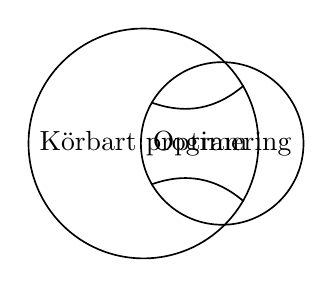
\begin{tikzpicture}[semithick]
            \node<3->[state](runinner) [] {Körbart program};
            \node<4->[state](optcomp)  [right of=runinner] {Optimering};
            \path<4->
              (runinner) edge[bend left] node {} (optcomp)
              (optcomp)  edge[bend left] node {} (runinner);
          \end{tikzpicture}
          Körning
        };
        \path (socker) edge            node {} (stg);
        \path (stg)    edge            node {} (int);
        \path<2-> (stg)    edge            node {} (comp);
        \path (haskell) edge           node {} (stg);
        \path<3-> (comp)   edge            node {} (run);
        \end{tikzpicture}
\end{figure}
\end{frame}

\begin{frame}
\begin{center}
\Large{http://github.com/simedw/Kandidat}
\end{center}
\end{frame}

\end{document}
